\chapter{A new low mach approach for Supercritical fluids}
\chaptertoc{}

A novel low-Mach-number algorithm for the thermal Lattice Boltzmann Method (LBM)
is developed to efficiently simulate supercritical fluid dynamics using
real-fluid thermodynamics. Unlike existing approaches, the proposed method
incorporates a conservative formulation compatible with cubic equations of state
(EoS), enabling accurate representation of strongly non-ideal behaviors typical
of supercritical conditions. A low-Mach number approximation is used to improve
computational efficiency without compro- mising physical fidelity. This
formulation retains mass, momentum, and energy conservation and extends the
applicability of LBM to regimes where classical ideal-gas-based models fail. The
algorithm is validated through canonical supercritical flow benchmarks,
demonstrating excellent agreement with reference data and significantly enhanced
numerical stability and per- formance.

\section{Ideal Gas EoS}

To enhance computational efficiency in thermally driven, weakly compressible
flows, several low Mach number (LMN) extensions of LBM have been proposed in
literature. Notable efforts include the work of Wang et al.~\cite{wang2022new},
who developed a LMN model for thermal flows of ideal gases, that of Hosseini et
al.~\cite{hosseini2023low}, who extended LBM to improve energy transport
modeling, and, finally, that of  Filippova and Hänel~\cite{filippova2000novel},
who introduced temperature coupling via source terms. However, to the best of
our knowledge, none of these LMN approaches have been applied to flows under
supercritical conditions using a real-fluid equation of state.

\section{A Conservative Low Mach Number Approach for supercritical fluid flows}

In many fluid dynamics problems, especially those involving supercritical
fluids, the Mach number can be very small. This occurs when the fluid velocity
is significantly lower than the speed of sound. From an eigenvalue analysis of
the Navier–Stokes equations, it is evident that the characteristic wave
propagation speeds are tied directly to the speed of sound. As a consequence, to
satisfy the Courant–Friedrichs–Lewy (CFL) condition, the time step required for
stable numerical integration becomes extremely small, rendering simulations
computationally expensive.

To overcome this challenge, several strategies have been proposed, such as the
Pressure Gradient Scaling (PGS) ~\cite{ramshaw1985pressure} method and the Low
Mach Number (LMN) approximation. The PGS method consists of artificially
modifying the speed of sound by scaling the pressure gradient. This modification
allows for larger time steps without violating the CFL condition.

This technique is well-suited for traditional Navier–Stokes solvers due to its
efficiency in computing macroscopic quantities. However, the PGS approach is
only valid in the absence of external force terms. When such forces are present,
the scaling of the pressure gradient alters the non-dimensional parameters of
the flow, potentially leading to incorrect physical
behavior~\cite{wang2004artificial}.

Several attempts have been made to adapt the LMN approach for LBM. However,
these have been mostly  to the ideal gas EoS and often fail to conserve mass
accurately, as the density is not consistently computed from the lattice
populations ~\cite{wang2022new, hosseini2023low}. In the following, the
mass-conserved low Mach number acceleration approach for EoS other than ideal
gas applied in the current work will be presented.

\subsection{Low Mach Number Expansion and Governing Equations}

The macroscopic equations derived from the LBM are equivalent to the
Navier–Stokes equations. The velocity, space coordinates, temperature and
density are made dimensionless by choosing respectively the characteristic
velocity, $U_0$, length, $L_0$, temperature, $T_0$, and density, $\rho_0$, of
the problem considered as reference values. They are obviously different for
each problem. The reference time and pressure are then chosen as $L_0/U_0$ and
$\rho_0 c_0^2$, with $c_0$ the speed of sound at the reference temperature,
respectively. The dimensionless equations then read:

\begin{equation}
    \frac{\partial \rho}{\partial t} + \frac{\partial (\rho u_\alpha)}{\partial x_\alpha}  = 0
\end{equation}

\begin{equation}
    \frac{\partial (\rho u_\alpha)}{\partial t}  + \frac{\partial (\rho u_\alpha u_\beta)}{\partial x_\beta} = -\frac{1}{M\!a^2} \frac{\partial P}{\partial x_\alpha } + \frac{1}{Re} \frac{\partial \mathcal{T}_{\alpha\beta}}{\partial x_\beta} + \frac{1}{Fr^2} \rho G_\alpha
\end{equation}

\begin{equation}
    \frac{\partial (\rho E)}{\partial t} + \frac{\partial (\rho u_\beta H)}{\partial x_\beta} = \frac{1}{Re\, Pr} \frac{\partial }{\partial x_\beta} (\lambda \frac{\partial T}{\partial x_\beta}) + \frac{1}{Re} \frac{\partial (u_\beta \mathcal{T}_{\alpha\beta})}{x_\beta} + \frac{1}{Fr^2} \rho G_\alpha u_\alpha
\end{equation}
where $Re$, $M\!a$, $Fr$ and $Pr$ are the Reynolds, Mach, Froude and Prandtl
numbers, respectively, defined by: 

\begin{equation*}
   Re = \frac{\rho_0 U_0 L_0}{\mu_0} , M\!a = \frac{U_0}{c_0} , Fr = \frac{U_0}{\sqrt{g L_0}} , Pr = \frac{\mu_0 C_{P0}}{\lambda_0} 
\end{equation*}
where $\mu_0$, $\lambda_0$ and $C_{P0}$ are the values of viscosity, thermal
conductivity and specific heat capacity, respectively, at the reference
temperature and density.

An expansion of the main variables is performed using the Mach number as a small
parameter:

\begin{align}
    \rho &= \rho^{(0)} + M\!a^2 \rho^{(1)} +o(M\!a^2) \\
    u_{\alpha} &= u_{\alpha}^{(0)} + M\!a^2 u_{\alpha}^{(1)} + o(M\!a^2) \\
    T &= T^{(0)} + M\!a^2 T^{(1)} + o(M\!a^2) \\
    P &= P^{(0)} + M\!a^2 P^{(1)} + o(M\!a^2)
\end{align}

 Substituting these expansions into the governing equations, after the
 multiplication of the momentum equation by $M\!a^2$, and neglecting terms of
 order $o(M\!a^2)$, the following reduced system was obtained:

\begin{equation}
    \frac{\partial \rho^{(0)}}{\partial t} + \frac{\partial (\rho^{(0)} u^{(0)}_\alpha)}{\partial x_\alpha} = 0
\end{equation}

\begin{align}
    M\!a^2 \frac{\partial (\rho^{(0)} u^{(0)}_\alpha)}{\partial t} 
    + M\!a^2 \frac{\partial (\rho^{(0)} u^{(0)}_\alpha u^{(0)}_\beta)}{\partial x_\beta}
    &= - \frac{\partial}{\partial x_\beta} 
        \left(P^{(0)}\delta_{\alpha\beta} + M\!a^2 P^{(1)}\delta_{\alpha\beta}\right) \nonumber \\
    &\quad + \frac{M\!a^2}{Re} \frac{\partial \mathcal{T}_{\alpha\beta}^{(0)}}{\partial x_\beta}
    - \frac{M\!a^2}{Fr^2}G_\alpha
\end{align}


\begin{equation}
    \frac{\partial (\rho^{(0)} E^{(0)})}{\partial t} + \frac{\partial (\rho^{(0)} u_\beta^{(0)} H^{(0)})}{\partial x_\beta} = \frac{1}{Re Pr} \frac{\partial }{\partial x_\beta} (\lambda^{(0)} \frac{\partial T^{(0)}}{\partial x_\beta}) + \frac{1}{Re} \partial_\alpha u_\beta^{(0)}\mathcal{T}_{\alpha\beta}^{(0)}
\end{equation}

The momentum equation reduces at $0^{th}$ order to $\partial
(P^{(0)}\delta_{\alpha\beta}) / \partial x_\beta=0$, which shows that the
leading order pressure $P^{(0)}$ only depends on time. At order
$\mathcal{O}(M\!a^2)$, the following is obtained: 

\begin{equation}
    \frac{\partial (\rho^{(0)} u^{(0)}_\alpha)}{\partial t} + \frac{\partial (\rho^{(0)} u^{(0)}_\alpha u^{(0)}_\beta)}{\partial x_\beta} = -\frac{\partial (P^{(1)}\delta_{\alpha\beta})}{\partial x_\beta} + \frac{1}{Re} \frac{\partial \mathcal{T}_{\alpha\beta}^{(0)}}{\partial x_\beta} - \frac{1}{Fr^2}G_\alpha
\end{equation}


So, solely the variables of order $\mathcal{O}(0)$ are computed except for the
pressure. The homogeneous pressure $P^{(0)}$ appears only in the energy equation
and in the EoS, that is why it is usually named as thermodynamic pressure, noted
$P_{th}$. The pressure of order $\mathcal{O}(M\!a^2)$, which is decorrelated
from the temperature, appears only in the momentum equation and represents the
contribution of hydrodynamics only. Since the hydrodynamic equations are solved
here through the LBM method, the pressure $P^{(1)}$ can be identified as the
classical pressure of the athermal LBM defined as: 

\begin{align}
    P^{(1)} &=  \rho^{(1)} c_s^2
\end{align}

In order to write $P = P_{th} + P_{dyn}$, the dynamic pressure $P_{dyn}$ is
defined by:

\begin{align}
    P_{dyn} &= M\!a^2 P^{(1)}
\end{align}


\subsection{Thermodynamic Pressure calculation}

The Low Mach Number approximation introduces an additional variable, the
thermodynamic pressure $P_{th}$. In open systems, this pressure is not only
homogenous in space but it is also constant in time. It is therefore set to its
value at time $t=0$. However, for closed systems, it must be calculated at each
time step. A classic approach consists of obtaining the thermodynamic pressure
from global mass conservation: 

\begin{equation}
    \int_V \rho(x,t) \, \mathrm{d}V = \int_V \rho(x,0) \, \mathrm{d}V
\end{equation}

The pressure–density relationship is defined by an EoS. In this work, the
Peng–Robinson EoS is employed, expressed as:
\begin{equation}
    P_{th} = \frac{\rho r T}{1 - b\rho} - \frac{a \rho^2}{1 + 2b\rho - b^2 \rho^2}
\end{equation}

This equation can be reformulated as :

\begin{equation}
    \rho = \frac{P_{th}}{(rT + b P_{th})(1 + 2b\rho - b^2 \rho^2) - a \rho(1 - b\rho)}
\end{equation}

Thus, the thermodynamic pressure at each time step is computed by solving:

\begin{equation}
    P_{th}(t) = \frac{\int_D \rho(x,0) \, \mathrm{d}D}{\int_D \frac{1}{(rT + b P_{th}(t))(1 + 2b\rho - b^2 \rho^2) - a\rho(1 - b\rho)} \, \mathrm{d}D}
\end{equation}

This equation can be solved iteratively, enabling accurate pressure computation
for complex EoS in a conservative LBM framework.


\subsection{Evolution equation for the dynamic Pressure}

%The dynamic pressure, as seen in the last section, is decorrelated from the
%temperature. Thus, the pressure of order $\mathcal{O}(1)$ can be identified as
%the classical pressure of the LBM and is defined as: 

%\begin{align} P^{(1)} &=  \rho^{(1)} c_s^2 \end{align}

%In order to write $P = P_{th} + P_{dyn}$, we include the Mach number in the
%definition of the dynamic pressure :

%\begin{align} P_{dyn} &= Ma^2 P^{(1)} \end{align}

For simulations based on the solution of the Navier-Stokes equations, the
classic strategy consists in deriving a Poisson equation for $P_{dyn}$ from the
momentum equation. Unfortunately, this approach is not interesting here since it
loses the explicit nature of the LBM method. However, an evolution equation can
be derived for the dynamic pressure from the continuity equation at order
$\mathcal{O}(M\!a^2)$, as demonstrated in ~\ref{appendix:2ndOrderMoments}, which
is valid for low Mach number:

\begin{equation}
    \frac{\partial P_{dyn}}{\partial t} + c_s^2 \frac{\partial}{\partial x_{\alpha}}(\rho u_\alpha - \rho^{(0)} u_\alpha^{(0)}) = 0
\end{equation}

From the continuity equation, it follows that:

\begin{align}
    \frac{\partial (\rho^{(0)} u_\alpha^{(0)})}{\partial x_\alpha} &= -\frac{\partial \rho^{(0)}}{\partial t}
\end{align}

The following evolution equation for the dynamic pressure is then obtained:

\begin{equation}
    \frac{\partial P_{dyn}}{\partial t} = c_s^2( -\frac{\partial (\rho u_\alpha)}{\partial x_\alpha} - \frac{\partial \rho^{(0)}}{\partial t})
\end{equation}
where $\partial (\rho u_\alpha) / \partial x_\alpha$ is computed from the LBM as
mentioned in ~\cite{wissocq2022restoring}. Thus, in order to achieve the time
evolution  of $P_{dyn}$,  the time derivative of the thermodynamic density is
needed. To this end, the parameter \(\theta\) in the uHRR-LBM method (see
\ref{appendix:uHRR-LBM}), defined by \(P = c_s^2 \rho \theta\), is considered, and an
expansion of \(\theta\) is performed as:

\begin{equation}
    \theta = \theta^{(0)} + M\!a^2 \theta^{(1)} +o(M\!a^2)
\end{equation}

Therefore, at order \(\mathcal{O}(0)\), the following equation is obtained:

\begin{equation}
    P_{th} = c_s^2 \rho^{(0)} \theta^{(0)}
\end{equation}

Then, deriving this equation with respect to time (and remembering that $P_{th}$
is independent on space) leads to :

\begin{equation}
    \frac{\mathrm{d} P_{th}}{\mathrm{d} t} = c_s^2 \theta^{(0)} \frac{\partial \rho^{(0)}}{\partial t}+ c_s^2 \rho^{(0)} \frac{\partial \theta^{(0)}}{\partial t}
\end{equation}

from which $\partial \rho^{(0)} / \partial t$ can be computed as :

\begin{equation}
    \frac{\partial \rho^{(0)}}{\partial t} = \frac{1}{c_s^2 \theta^{(0)}} \left[ \frac{\mathrm{d} P_{th}}{\mathrm{d} t} - c_s^2 \rho^{(0)} \frac{\partial \theta^{(0)}}{\partial t} \right]
\end{equation}

\hspace{2cm}

To summarize a simplified flow chart of the algorithm is presented in Figure
\ref{Flow Chart}.

\begin{figure}[ht!]
\centering
\includegraphics[width=0.7\columnwidth]{FlowChart3.png}
\caption{Flowchart of the simulation algorithm.}
\label{Flow Chart}
\end{figure}

\section{Validation test cases}

In this section, various test cases are presented to validate the LMN
formulation of the model. In all cases, supercritical conditions are ensured by
selecting pressure and temperature values above the gas-liquid critical point.
The Peng-Robinson EoS is employed throughout the simulations. All the test cases
are performed using a two-dimensional computational domain, with the exception
of the Mayer’s jet test case, which is conducted in three dimensions.

\subsection{Entropy spot}
The entropy spot test is a well-established benchmark in fluid dynamics used to
assess the accuracy and stability of numerical methods, particularly for
low-Mach-number flows. It involves initializing a localized density perturbation
in a quiescent fluid and tracking its evolution under Eulerian conditions, where
no diffusion or damping is expected. The initial density field is defined by:

\begin{equation}
    \rho = \rho_0 \left(1 + \epsilon\, e^{-r^2/R^2} \right)
\end{equation}

where $\rho_0 = 543\ \mathrm{kg/m^3}$ $\rho_0 = 543\si{kg/m^3}$, $\epsilon =
0.01$, $R = 0.1$. The radial distance is defined as $r = \sqrt{(x - x_c)^2 + (y
- y_c)^2}$, where $(x_c, y_c)$ are the coordinates of the entropy spot's center
. The fluid used is supercritical carbon dioxide (\ce{CO2}), initialized at a
pressure of $90\ \mathrm{bar}$. The simulation is performed over five periods
and with periodic boundary conditions, for a Mach number of $M\!a = 0.00348$
ensuring compressibility effects remain small but measurable.

To assess spatial accuracy, four mesh resolutions were tested: $100\times100$,
$200\times200$, $400\times400$, and $800\times800$. The energy equation is
integrated using the 2D MUSCL-Hancock scheme~\cite{wissocq2022restoring}, which
theoretically achieves third-order accuracy.

Results are shown in Fig.~\ref{fig: Entropy LMN} demonstrating convergence to
the analytical solution. The LMN solver shows only second-order convergence,
which aligns with theoretical expectations for Lattice Boltzmann Methods.

A key advantage of the LMN formulation is its computational efficiency. Due to
the larger allowable time steps up to 15 times larger than those in the FC
solver. The LMN approach significantly reduces simulation cost while maintaining
excellent accuracy.

\begin{figure}[htpb]
    \centering
    \includegraphics[width=\columnwidth]{LMN_entropy_spot.pdf}
    \caption{Comparison of analytical and LMN simulation results for an entropy spot of supercritical \ce{CO2}.}
    \label{fig: Entropy LMN}
\end{figure}
    
    
\begin{figure}[htb]
    \centering
    \includegraphics[width=\columnwidth]{L2Error.pdf}
    \caption{L2 error in density field for the entropy spot}
    \label{L2 error}
\end{figure}

\subsection{Poiseuille flow}
Poiseuille flow describes steady, laminar motion of a viscous fluid between
parallel plates under a horizontal pressure gradient. It exhibits a parabolic
velocity profile and serves as a benchmark for validating numerical solvers.

In this study, supercritical \ce{CO2} flows between two parallel plates
separated by a distance of \(H = 0.1\,\text{mm}\). The fluid is initialized at
90\,bar and 310\,K. Under these conditions, sCO\textsubscript{2} exhibits a
liquid-like, nearly incompressible, behavior. %, with a speed of sound of
approximately $c = 286.95$\,m/s. The dynamic viscosity is $\mu = 3.89 \times
10^{-5}$\,Pa$\cdot$s. 
The maximum value of the Mach number in the simulations is 2.49 $\times 10^{-5}$
confirming the low-Mach number regime and justifying the incompressibility
assumption in this configuration. A Reynolds number of 8 is employed, ensuring
laminar flow. 

The analytical velocity profile is:

\begin{equation}
u(y) = u_{\text{max}} \left( \frac{4y}{H} - \frac{4y^2}{H^2} \right),
\end{equation}

where $u(y)$ is the horizontal velocity as a function of vertical coordinate
$y$.

As shown in Fig.~\ref{fig:poiseuille}, the LBM simulations, whether they are
based on the fully compressible approach or the LMN formulation, closely match
the analytical solution, validating our numerical solvers in supercritical,
low-Mach number conditions.


\begin{figure}[htb]
\centering
\includegraphics[width= \columnwidth]{poisseuille.pdf}
\caption{Comparison of analytical and LBM simulation results for Poiseuille flow
of supercritical CO\textsubscript{2}.}
\label{fig:poiseuille}
\end{figure}

\subsection{Double shear layer in Mayer's jet condition}
The simulation setup follows a two-dimensional Double Shear Layer (DSL)
configuration. The solution is initialized with prescribed temperature,
pressure, and velocity fields over a square region of side length \(L\), using
periodic boundary conditions. This setup is adapted to replicate the conditions
of Mayer’s jet experiment, specifically case 3 as described
in~\cite{mayer2003raman, petit2013large}. All relevant geometric and physical
parameters used in the simulation are summarized in
Tab.~\ref{tab:mayer_combined}.

\begin{table*}[htbp]
    \centering
    \caption{Parameters used for Mayer’s Jet Cases 3 and 4}
    \label{tab:mayer_combined}
    \renewcommand{\arraystretch}{1.2}
    \begin{tabular}{llccr}
        \toprule
        \textbf{Parameter} & \textbf{Symbol} & \textbf{Case 3} & \textbf{Case 4}
        & \textbf{Unit} \\
        \midrule
        \multicolumn{5}{l}{\textbf{Geometrical parameters}} \\
    
        %Jet length           & $L_{inj}$                   & 250   & 6.6   & mm
        %\\
        Injector diameter    & $D_{inj}$               & 2.2   & 2.2   & mm \\
        \midrule
        \multicolumn{5}{l}{\textbf{Case-specific flow parameters}} \\
        Ambient pressure     & $P_\infty$              & 39.7  & 39.8  & bar \\
        Ambient temperature  & $T_\infty$              & 298.0 & 298.0 & K \\
        Injection temperature& $T_{inj}$               & 126.9 & 137.0 & K \\
        Injection velocity   & $U_{inj}$               & 4.9   & 5.4   & m/s \\
        \bottomrule
    \end{tabular}
\end{table*}


Figure~\ref{DSL} illustrates the simulation domain, where subscripts \(inj\) and
\(\infty\) refer to jet and ambient (reservoir) conditions, respectively. The
parameter \(\alpha\), which defines the fraction of the domain’s width occupied
by the cold layer, was fixed at \(\alpha = 1/3\) for all simulations.

\begin{figure}[htb]
    \centering
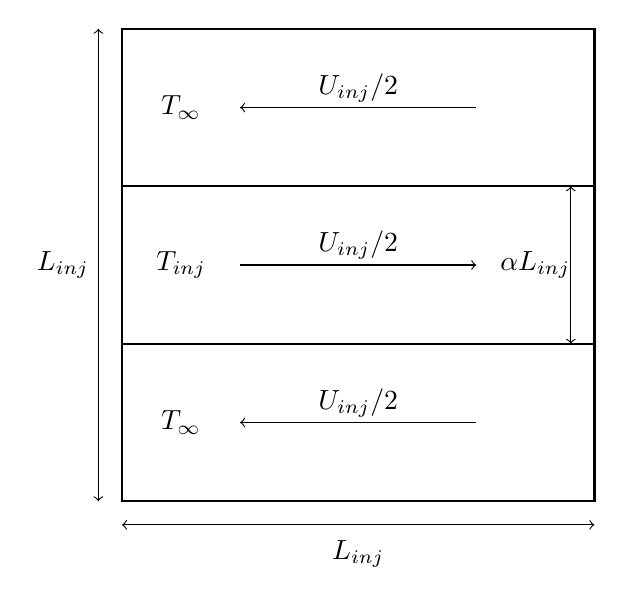
\begin{tikzpicture}

% Define the size of the square
\def\L{6}

% Draw the outer square
\draw[thick] (0,0) rectangle (\L,\L);

% Define the height of each region
\def\regionHeight{\L/3}

% Draw the horizontal lines to divide the square into three regions
\draw[thick] (0,\regionHeight) -- (\L,\regionHeight); \draw[thick]
(0,2*\regionHeight) -- (\L,2*\regionHeight);

% Label the regions
\node at (\L/2, \regionHeight/2+\regionHeight/8) {$U_{inj}/2$}; \node at (\L/2,
\regionHeight + \regionHeight/2 + \regionHeight/8) {$U_{inj}/2$}; \node at
(\L/2, 2*\regionHeight + \regionHeight/2 + \regionHeight/8) {$U_{inj}/2$};

% Label of temperature
\node at (\L/8, \regionHeight/2) {$T_\infty$}; \node at (\L/8, \regionHeight +
\regionHeight/2) {$T_{inj}$}; \node at (\L/8, 2*\regionHeight + \regionHeight/2)
{$T_\infty$};

% Label of dimenssions
\node at (-\L/8, 3*\regionHeight/2) {$L_{inj}$}; \node at (7*\L/8,
3*\regionHeight/2) {$\alpha L_{inj}$}; \node at (\L/2, -\regionHeight/3  )
{$L_{inj}$};

% Optional: Add arrows to indicate flow direction
\draw[->] (\L/4 + \L/2, \regionHeight/2) -- (\L/4, \regionHeight/2); \draw[->]
(\L/4, \regionHeight+\regionHeight/2) -- (\L/4 + \L/2, \regionHeight +
\regionHeight/2); \draw[->]  (\L/4 + \L/2, 2*\regionHeight + \regionHeight/2)--
(\L/4, 2*\regionHeight + \regionHeight/2);

% Add arrows to indicate dimensions
\draw[<->] (0, -\L/20) -- (\L, -\L/20); \draw[<->] (-\L/20, 0) -- (-\L/20 , \L);
\draw[<->] (\L - \L/20, \L/3) -- (\L -\L/20 , 2*\L/3);
\end{tikzpicture}
\caption{Double shear layer configuration}
\label{DSL}
\end{figure}

The imposed pressure for the whole domain $P_\infty$ and velocity $U_{inj}$ are
respectively set to $P_\infty = 39.7$ bar and $U_{inj}= 4.9$ m.s$^{-1}$ in order
to match Mayer’s jet pressure and shear stresses between both pseudo-phases. Jet
and ambient temperatures are also matched to Mayer jet’s: $T_\infty$ = 298 K and
$T_{inj}$ = 126.9 K. Corresponding thermodynamic variables are computed via
Peng-Robinson EoS.

For the initialization, a function $\phi$ is defined as follows:
\begin{equation}
    \phi(y) = 1-\tanh\left[ \frac{(R-R_0)}{\delta_0}\right] \times \frac{1}{2}
\end{equation}
where $R_0$ corresponds to the radius of the injection inlet and $\delta_0$ was
fixed to $1.5\times 10^{-4}$. Then the velocity and the temperature are defined
as follows:

\begin{equation}
    u_x(y) = \frac{u_0}{2}\phi  - \frac{u_0}{2}(1-\phi)
\end{equation}
 
\begin{equation}
    T(y) = T_\infty\phi + T_j(1-\phi)
\end{equation}

Additionally, in order to trigger instabilities, an orthogonal perturbation
velocity of magnitude $\epsilon = 5 \% $ of $u_0$ and spatial period $L$, is
introduced along the x-axis:

\begin{equation}
    u_y(x)=\epsilon u_0 \sin\left(2\pi\frac{x}{L}\right)
\end{equation}

The simulations are performed for two convective times, defined as \(\tau_c =
u_0 / L\). The resulting density fields are presented in Fig.~\ref{fig:FC_DSL}
and Fig.~\ref{fig:LMN_DSL} for the FC and LMN approaches, respectively. A
diagonal line is drawn from the bottom-left to the top-right corner in each
figure to analyze the density variation along this direction. The corresponding
one-dimensional density profiles extracted along this diagonal are shown in
Fig.~\ref{Density_DSL_FC} and Fig.~\ref{Density_DSL_LMN}, again for the FC and
LMN cases, respectively.

\begin{figure*}[htbp]
    \centering
    \subfloat[Density field  FC]{%
        \includegraphics[width=6.25cm]{FC_DSL.pdf}%
        \label{fig:FC_DSL}%
    }\hfill \subfloat[Density field LMN]{%
        \includegraphics[width=6.25cm]{LMN_DSL.pdf}%
        \label{fig:LMN_DSL}%
    }\hfill \subfloat[Density along diagonal FC]{%
        \includegraphics[width=6.25cm]{Density_FC_DSL(1).pdf}%
        \label{Density_DSL_FC}%
    }\hfill \subfloat[Density along diagonal LMN]{%
        \includegraphics[width=6.25cm]{Density_LMN_DSL(1).pdf}%
        \label{Density_DSL_LMN}%
    }\hfill \caption{ Density fields (a, b) and corresponding diagonal profiles
    (c, d) for the FC and LMN approaches after two convective times (\(\tau_c =
    u_0 / L\)). }
    \label{DSL_LMN and FC}
\end{figure*}

Different mesh resolutions were analyzed for both the LMN and FC solvers.
Notably, the simulations remained stable even on a relatively coarse mesh
(64×64). It is important to highlight that no sensor-based viscosity was applied
in this test case; thus, the observed stability is entirely attributed to the
numerical viscosity and hyperviscosity arising from truncation errors, similar
to the results found by ~\cite{farag2021unified} for the ideal gaz.

The three previous test cases demonstrate an excellent agreement between the FC
and the LMN solutions. Therefore, in the subsequent simulations, only the LMN
algorithm is applied, as it is significantly faster.

\subsection{Natural Convection of Supercritical \ce{CO2}}

The problem of natural convection in a 2D differentially heated cavity is a
benchmark case study used for many years for the validation of computational
codes (see for example the paper of Le Quéré et al.~\cite{Lequere2005} for the
validation of Low Mach number algorithms for perfect gas). The LMN solver is
compared with a spectral code~\cite{Ameur2013} for this benchmark problem
involving supercritical \(\ce{CO2}\). The simulation is conducted at a pressure
of \(P = 2 P_c\), where \(P_c = 73.7 \) bar is the critical pressure of
$\ce{CO2}$. The cavity has a height of 2.8 mm, with the left and right walls
maintained at 335.97 K and 334.97 K, respectively. The horizontal walls are
adiabatic.

Under these conditions, the fluid operates in the pseudo-boiling region, where
thermodynamic properties vary sharply due to the proximity to the inflection
point of the cubic equation of state (EoS). In particular, the thermal expansion
coefficient differs significantly from that predicted by the ideal gas EoS,
impacting the flow structure since the Rayleigh number is much larger than for a
perfect gas. 

To match the accuracy of the spectral solution (grid resolution \(141 \times
141\)), a uniform cartesian mesh of \(1128 \times 1128\) was used for the LBM.
This resolution is consistent with the finer near-wall resolution typically
achieved by spectral methods, which is critical for accurate heat transfer
prediction.

Figure~\ref{fig:RB_temperature} presents the spatial distribution of the
temperature field. Remarkably, despite a temperature difference of only 1~K
between the cold and hot walls, the resulting temperature profiles exhibit
shapes typically observed in ideal gas simulations at high Rayleigh numbers,
such as those reported in~\cite{wang2022new}, where the temperature difference
between the walls was 720~K. This behavior arises due to the unique
thermophysical properties of supercritical \ce{CO2} in the pseudo-boiling
region, especially the high thermal expansion coefficient and low viscosity,
leading to a Rayleigh number equal to $ 10^6$. 

\begin{figure}[H]
\centering
\includegraphics[width=\columnwidth]{RBCountour.pdf}
\caption{Temperature distribution of supercritical $\ce{CO2}$ inside the
cavity.}
\label{fig:RB_temperature}
\end{figure}

In Fig.~\ref{fig:RB_validation}, the Nusselt number profiles at the cold and hot
walls are presented. The red solid lines correspond to the spectral solution,
while the black dashed lines represent the results from the LMN solver. The
agreement between the two methods is excellent, with only a 1\% difference in
the global Nusselt number. The discrepancy observed on the maximum values near
the top and bottom walls corners may be attributed to the high spatial
resolution of the spectral method near the boundaries, since the calculation
points density is naturally larger there, which allows for more accurate capture
of thermal boundary layer effects. Moreover, as is well documented in the
literature ~\cite{kruger2017lattice}, the LBM can face challenges in accurately
resolving flow features in corner regions.


\begin{figure}[htbp]
\centering
\includegraphics[width=\linewidth]{RB1122x1122.pdf}
\caption{Profiles of the Nusselt number at the two thermostated vertical walls
for natural convection of supercritical $\ce{CO2}$: Comparison between LBM and
spectral solvers.}
\label{fig:RB_validation}
\end{figure}

Figures~\ref{fig:RB_temp_profiles} and~\ref{fig:RB_velocity_profiles} show the
temperature and velocity profiles at the mid-height of the cavity, respectively.
The results demonstrate good agreement with the reference spectral solution,
especially for temperature. As observed for the Nusselt number, the velocity
profiles exhibit discrepancies in the boundary layers along the heated and cold
walls, likely due to the high resolution of the spectral method near the
boundaries whereas LBM uses a uniform Cartesian mesh. 

\begin{figure}[htbp]
\centering
\includegraphics[width=0.8\linewidth]{RBTempCO2.pdf}
\caption{Temperature profiles at mid-height of the cavity for natural convection
of supercritical $\ce{CO2}$: Comparison between LBM (1128×1128) and spectral
(141×141) solvers.}
\label{fig:RB_temp_profiles}
\end{figure}

\begin{figure}[H]
\centering
\includegraphics[width=0.8\linewidth]{RBVyCO2.pdf}
\caption{Vertical velocity profiles at mid-height of the cavity for natural
convection of supercritical $\ce{CO2}$: Comparison between LBM (1128×1128) and
spectral (141×141) solvers.}
\label{fig:RB_velocity_profiles}
\end{figure}


\subsection{Flow Around a Circular Cylinder at \texorpdfstring{$Re = 100$}{Re =
100}}

This test case is well established in the field of aerodynamics, where the
primary condition to be satisfied is the Reynolds number. To the best of the
authors' knowledge, this specific configuration has been previously investigated
only using ideal gas equations of state. However, according to the Buckingham
\(\Pi\)-theorem, the governing physics of a flow remain unchanged as long as the
relevant dimensionless numbers are matched, regardless of the working fluid. For
this reason, this case can confidently be used to validate simulations with
supercritical \(\ce{CO2}\), provided that the Mach number remains low and the
Reynolds number is set to \(Re = 100\).

This test case evaluates the performance of the LBM model for unsteady, weakly
compressible flow past a circular cylinder. The Reynolds number is fixed at \(Re
= 100\), and the flow is simulated at a low Mach number, \(M\!a_\infty = 0.1\),
to minimize compressibility effects.

The cylinder, with a diameter \(D = 80\,\Delta x\), is centered at the origin
\((0, 0)\) within a rectangular computational domain defined by \([{-}25D, 75D]
\times [{-}30D, 30D]\), discretized using a uniform Cartesian mesh. A uniform
inflow is imposed along the \(x\)-axis with velocity :
\[
U_\infty = M\!a_\infty c_\infty,
\]
where \(c_\infty\) is the free-stream speed of sound. A no-slip boundary
condition is enforced on the surface of the cylinder.

At \(Re = 100\), the flow develops periodic vortex shedding, characterized by
the Strouhal number:
\[
St = \frac{f_{\text{req}} D}{U_\infty},
\]
where \(f_{\text{req}}\) is the vortex shedding frequency. Aerodynamic forces
are computed using the immersed boundary force method, in which the effective
surface area is defined as \(S_{\text{eff}} = D \times \Delta
x\)~\cite{cheylan2022analysis}.

The computed drag, lift, and Strouhal numbers are compared against benchmark
data in Tab.~\ref{tab:Re100}, showing excellent agreement with results from
previous numerical studies. Minor discrepancies observed in the literature are
often attributed to differences in numerical methods; however, as discussed
earlier, the essential physics remain unchanged when the key dimensionless
numbers are preserved, even when using supercritical \ce{CO2} instead of an
ideal gas.

\begin{figure}[H]
\centering
\includegraphics[width=0.8\columnwidth]{CylinderLMNARe100.png}
\caption{Velocity field for supercritical \ce{CO2} flow around a cylinder at
\(Re = 100\), \(M\!a = 0.1\).}
\label{fig:cylinder_velocity}
\end{figure}

\begin{table}[ht]
    \centering
    \renewcommand{\arraystretch}{1.2}
    \begin{tabular}{|l|c|c|c|}
        \hline
        \textbf{Study} & \textbf{$C_d$} & \textbf{$C_l$} & \textbf{$St$} \\
        \hline
        Gsell and Favier (IBM) ~\cite{gsell2021direct}         & 1.37 & $\pm
        0.340$ & 0.164 \\
        Cheylan et al. (2022, IBM) ~\cite{cheylan2022analysis} & 1.41 & $\pm
        0.330$ & 0.166 \\
        Ménez et al. (2023, IBM) ~\cite{menez2023assessment}   & 1.36 & $\pm
        0.297$ & 0.161 \\
        Liu, Zheng, and Sung ~\cite{liu1998preconditioned}     & 1.35 & $\pm
        0.339$ & 0.164 \\
        Zhou, So, and Lam ~\cite{zhou1999vortex}               & 1.49 & $\pm
        0.248$ & 0.162 \\
        Kim, Kim, and Choi ~\cite{kim2001immersed}             & 1.33 & $\pm
        0.320$ & 0.165 \\
        Bourguet and Lo Jacono ~\cite{bourguet2014flow}        & 1.32 & $\pm
        0.320$ & 0.164 \\
        present                                               & 1.42 & $\pm
        0.340$ & 0.165 \\
        \hline
    \end{tabular}
    \caption{Comparison of drag coefficient (\(C_d\)), lift coefficient amplitude (\(C_l\)), and Strouhal number (\(St\)) for \(Re = 100\).}
    \label{tab:Re100}
\end{table}


\subsection{Simulation of Mayer's Jet Case 4}

This study simulates Case 4 (see Tab.~\ref{tab:mayer_combined}) from the
experimental work of Mayer et al.~\cite{mayer2003raman}, involving the injection
of a free nitrogen jet under supercritical conditions. The primary objective is
to numerically reproduce the spatial evolution of density to validate the
results against experimental measurements obtained using two-dimensional Raman
spectroscopy.

In this test case, liquid nitrogen is injected into a chamber maintained above
its critical pressure. Under such conditions, both the injected jet and the
surrounding environment are in a supercritical state. The initial conditions are
summarized in Table~\ref{tab:mayer_combined}. The simulation uses a uniform grid
with spacing $\Delta x = \Delta y = \Delta z = 1.0\times 10^{-4}$~m and a time
step of $\Delta t = 8.25\times 10^{-7}$~s. The injector has a diameter of $D =
2.2\times 10^{-3}$~m and is located at the origin $(0,0)$. The computational
domain spans $[-10D,10D]\times[-10D,10D]\times[0,70D]$. A constant inlet
velocity of $4.9$~m/s is imposed, while all other boundaries are treated as
outlets with a Neumann condition, allowing fluid to exit the domain.

The analysis focuses on the near-field region ($x/D \leq 28.5$), which
corresponds to the range covered by the available experimental measurements.


Figure \ref{Density Field Mayer Cas 4} shows a comparison between the density
gradient variation obtained in our simulation and the experimental data. It can
be noted that the simulation correctly reproduces the zones of large density
gradients at the jet interface. 

\begin{figure}[H]
    \centering
    \subfloat[Experimental (Mayer et al.~\cite{mayer2003raman})]{%
        \includegraphics[width=6.25cm]{MayerExperimentalTest.png}%
        \label{fig:subfig11}%
    }\hfill \subfloat[Numerical simulation]{%
        \includegraphics[width=5.7cm]{Mayer4Numerical.png}%
        \label{fig:subfig12}%
    }\hfill
    \caption{Comparison of experimental and numerical density gradient field for Case 4 of Mayer's jet.}
    \label{Density Field Mayer Cas 4}
\end{figure}

Figure~\ref{Mayers jet cas 4} presents a quantitative comparison of
time-averaged centerline density obtained from various references using
different EoS, alongside the results from the present LMN solver. As shown, our
simulation demonstrates excellent agreement with the experimental data. Among
the numerical results, those reported by Mayer~\cite{mayer2003raman} are the
closest to ours, which is expected since his simulations employs an
incompressible formulation, making them compatible with the LMN approach used in
this work.


\begin{figure}[htpb]
\centering
\includegraphics[width=\columnwidth]{DensityCas4Mayer.pdf}
\caption{Comparison of experimental and numerical results of the average density for the Case 4 of Mayer's Jet. }
\label{Mayers jet cas 4}
\end{figure}